\begin{figure}
	\centering
	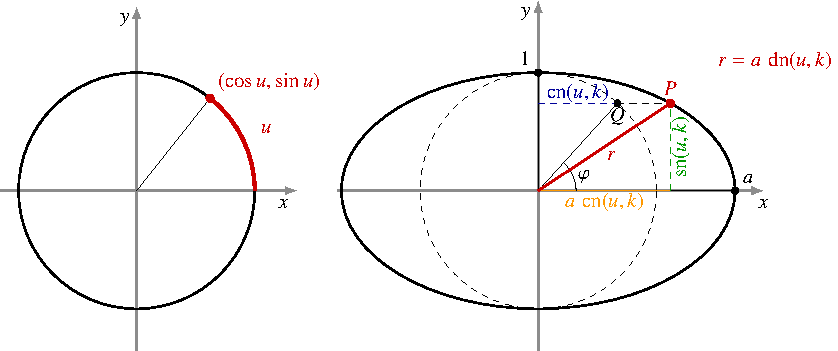
\includegraphics[width=0.7\textwidth]{papers/elliptisch/images/sn-konstruktion.pdf}
	\caption{Links der Einheitskreis mit dem Punkt $(\cos u, \sin u)$
	zur Bogenlänge $u$.
	Rechts die Ellipse mit den Halbachsen $a = 1/k'$ und $1$ zum
	selben Parameter, hier $u = 1$ und $k = 0.8$.
	Der Hilfskreispunkt
	$Q = (\operatorname{cn}(u,k), \operatorname{sn}(u,k))$
	und der Ellipsenpunkt
	$P = (a\operatorname{cn}(u,k), \operatorname{sn}(u,k))$
	liegen auf gleicher Höhe, der Abstand von $P$ zum Nullpunkt ist
	$r = a\operatorname{dn}(u,k)$. \cite[Kapitel~11.2.1]{elliptisch:mueller-spezielle} \cite{elliptisch:schwalm}
	\label{fig:elliptisch:snkonstruktion}}
\end{figure}
